\appendix
\section{MDP and SMDP}
\subsection{Introduction to MDP and the related terminologies}



Markov Decision Processes forms the crux for most of RL Research. In probability theory, Markov model is a stochastic model that models randomly changing systems with an underlying assumption that the future states depend only on the current state and not the events before that. As there is no dependence on history, the Markov models tend to provide a naive simplistic framework for RL Research. In the RL arrangement, a Markov Decision Process (MDP) is defined by a finite set of states \(\mathcal{S}\), a set of admissible actions for each state \(\mathcal{A}_s\), a real-valued reward function for each state-active pair \(R(s,a)\) and the transition probabilities \(P(s' \mid s,a)\). The MDP problem can be formulated as given: an agent observes a systems state \(s\), contained in \(\mathcal{S}\) and executes an action a as selected from \(\mathcal{A}_s\). An immediate reward with expected value of \(R(s,a)\) is yielded for this action. The agent moves to the next state  \(s'\), with a transition probability of \(P(s' \mid s,a)\). Note that if the problem was not MDP, then the transition probability would have also depended on the history rather than just \(s,a\). As the future reward depends only on one step (current state), this model is also known as the one-step model. We can think of collectively putting the flow of actions and states in a stochastic automaton. 


Consider a humanoid robot whose task is to open the door. This task can be further broken down into smaller primitive actions like reaching, holding and turning the knob. Assume that currently the robot is ten steps away from the door. Then the action which the robot most likely takes would be reaching out to the door. This action is not determined by any of the previous positions of the robot. For every state, the robot has a fixed set of possible actions. The robot chooses each of those actions with some specific probability given by the policy function. On choosing the action, the robot gets a reward. In this case, turning the knob would yield a reward of \(+1\), a reward of \(0\) for holding the knob and \(-1\) for every other case. This is a simple example of Markov Model. Note here that in RL, negative rewards are also rewards; this is based on the philosophy that a negative reward gives a learning experience to the agent, which is indeed a payoff. 


The policy function mentioned for the open-the-door example is a state-action mapping. In a deterministic world, it is given by \(\pi:\mathcal{S}_t \rightarrow \mathcal{A}_t\). It determines the action which can be taken from the given state at time-step \(t\). However, in a stochastic environment, the exact actions cannot be predicted. For this reason, a stochastic policy is given by \(\pi:\mathcal{S}_t \times U_{s \in \mathcal{S}} \mathcal{A}_{s_t} \rightarrow [0,1]\). It gives the probability of choosing an action \(a\), from a given state. Further, the RL literature assumes that the policies are stationary. In other words, the policy for a state-action pair does not vary with time. Hence, the Markov policy function is the stochastic stationary policy which gives the probability of choosing an action from a given state. The aim of the agent is to learn the best policy mapping for the given problem. The futuristic reward for choosing a state-action pair acts as the heuristic in determining the optimal policy. This futuristic reward is given by either the value function, \(V^\pi\) or the action-value function, \(Q^\pi\).  

For any policy \(\pi\) and state \(s\), \(V^\pi (s)\) is the value function, obeying policy \(\pi\). It denotes the expected return from \(s\), given that the agent uses policy \(\pi\). Return \(\mathcal{G}_t\), is the total reward obtained from the future steps. When the number of stages (iterations), is finite, then the total reward makes sense. However, in infinite-horizon cases, discounted return is considered. Discounted return gives more importance to the immediate rewards and a decaying weight to those which follow the reward. Thus, the policy function for MDP is the expected discounted-return. Let \(t\) denotes the time-step of the current stage. Consider \(s_t\) as the current state and \(r_(t+1)\) as the immediate reward for acting at stage \(s_t\) using policy \(\pi\). Then, the value function is defined as follows:

\begin{equation}
    V^\pi (s)=E[r_{t+1}+\gamma r_{t+2}+ \gamma^2 r_{t+3} + \dots \mid s=s_t,\pi]
\end{equation}

where \(0 \leq \gamma  \leq 1\), is the discount factor. When \(\gamma=0\), only the immediate reward is considered. When \(\gamma=1\), all the rewards are equally important. To learn the policy function, an optimal policy function must be learned. The unique optimal value function, \(V^*\), which maximizes the value of each state, is the value function corresponding to the optimal policy. 

We had seen that apart from value function, the action-value function also aids in determining the optimal policy. Given a policy \(\pi\), current state \(s\) and an action chosen for the current state \(a\), the action-value denoted by \(Q^\pi (s,a)\), is the expected infinite-horizon discounted return for choosing action \(a\) in state \(s\). It evaluates how good an action is for a given state. On the other hand, a value function \(V^\pi\) determines how favorable the current state is. Analogous to the value function, a action-value function is defined as follows:

\begin{equation}
    Q^\pi (s, a)=E[r_{t+1}+\gamma r_{t+2}+ \gamma^2 r_{t+3} + \dots \mid s=s_t, a=a_t, \pi]
\end{equation}

The optimal action-value, \(Q^*\) function maximizes the action-values for each state-action pair and yields the optimal policy. 

\subsection{Bellman Equations for Value and Action-Value Functions in MDP}

To learn optimal policies, optimal value and action-value functions must be learned. To converge to these optimal functions, we first re-write the \(V^\pi\) and \(Q^\pi\) functions. Let the current state be \(s\). Let \(a\) be executed from \(s\) to get a reward of \(R(s,a)\) for reaching the state \(s'\), with a transition probability of \(P(s' \mid s,a)\). We know that, the value function is the sum of the immediate reward obtained \(R(s,a)\) and a discounted sum of the future returns. The future returns can be thought of as the value function of state \(s'\), \(V^\pi (s')\).  The value for state \(s\) can be defined as:

\begin{equation}
    V^\pi (s)=\sum_{a \in \mathcal{A}_s} \pi(s,a)[R(s,a)  + \gamma \sum_{s'} P(s'\mid s,a) V^\pi (s')]
\end{equation}

The maximum value for a state is the maximum return obtained as compared to all the admissible actions. 


\begin{equation}
    V^* (s)=   \max_{a \in \mathcal{A}_s } ⁡R(s,a)  + \gamma \sum_{s'} P(s' \mid s,a) V^* (s')
\end{equation}

Similarly, there exists equations for \(Q^*\).

\begin{equation}
    Q^* (s,a)=R(s,a)+\gamma \sum_{s'} P(s'\mid s,a)   \max_{a' \in \mathcal{A}_{s'}}  ⁡Q^* (s',a')]    
\end{equation}


Given \(V^*\) and \(Q^*\), the optimal policy assigns a non-zero probability to those actions that maximize the value of that state. \(V^*\) and \(Q^*\) can further be learned using different strategies. Both \(V^*\) and \(Q^*\) can be re-written as:

\begin{equation}
    V^* (s)=\max_a ⁡Q^* (s,a)
\end{equation}

\begin{equation}
    Q^* (s,a)=R(s,a)+ \gamma \sum_{s'} P(s'\mid s,a)  V^* (s' ) 
\end{equation}


From these equations, it is evident that given \(V^*\), the reward and transition probabilities from the one-step model are not required to compute \(Q^*\). Thus, the action-value functions are much more important than the value-functions. Hence, rather than learning both \(V^*\) and \(Q^*\), just the Q-value is learnt for learning the optimal policy. Note that this learning just derives the optimal policy without explicitly learning the model (reward functions and the transition probabilities) and hence, it is a model-free approach. 


\subsection{Learning Q-value}

Approximation (also known as value-iteration) happens to be one of the naive ways for learning the Q-value. Consider Q-value iteration, which successfully updates \(Q^*\). For the sake of convenience, \(Q^\pi\) is represented simply by \(Q\) henceforth. At each iteration \(k\), it updates an approximate of \(Q_k\) of \(Q^*\) by applying the following operation for each state-action pair:

\begin{equation}
    Q_{k+1} (s,a)=R(s,a)+ \gamma \sum_{s' \in \mathcal{S}} P(s'\mid s,a)   \max_{a' \in \mathcal{A}_{s'}} ⁡Q_k (s',a')
\end{equation}

Starting with an arbitrary value of \(Q_0\), a sequence of such iterations converges to \(Q^*\). Such simple approximations do not work for most of the RL problems. The reason being that these algorithms learn the policies that are close to optimal ones over the entire state-space. However, a high precision need not be needed in states that are rarely visited. There are other learning algorithms like Q-learning and Sarsa, which give different importance to state-action pairs at different stages to combat this disadvantage of naive approximation. 


Q-learning algorithm is a simple value-iteration update, using a weighted average of the old value and new information. The update using Q-learning is defined as follows:

\begin{equation}
    Q_{k+1} (s,a)=(1-\alpha_k ) Q_k (s,a)+\alpha_k[R(s,a)+\gamma   \max_{a' \in \mathcal{A}_{s'}}⁡ Q_k (s',a' )]
\end{equation}

Where \(\alpha_k\) is the learning-rate parameter, \(0 < \alpha \leq 1\). The learning-rate determines up to what extent will the new information over-ride the older one. If \(\alpha=0\), then the agent will not learn anything. If \(\alpha=1\), then the agent prioritizes the most recently seen information. In this approach, the agents policy does matter as since the agents performance throughout the learning process is of interest. In other words, the agents policy influences the quantity to be maximized in the right-hand side of the equation. 

Sarsa is similar to Q-learning, except that the maximum action-value is replaced by the actual action-value at the next state.



\subsection{SMDP}

In hierarchical RL, the solutions to sub-problems are themselves considered as actions. Different actions can take different time to execute. In an MDP, the amount of time taken for an action to execute is not considered. A Semi Markov Decision process (SMDP) is defined like a MDP with an additional factor of \(\tau\), a random variable denoting the time elapsed between decision stages. \(\tau\) can both be real-valued and discrete valued. Most hierarchical RL frameworks use the discrete-time SMDP formulation. 

The transition probabilities \(P(s', \tau \mid s,a)\) in SMDP depicts the joint probability of an agent transiting from state \(s\) to state \(s'\)  after \(\tau\) time-steps by executing action \(a\). The expected rewards \(R(s,a)\) denotes the reward accumulated by executing action \(a\) in state \(s\) and waiting for \(\tau\) time-steps. The Bellman equations for \(V^*\) and \(Q^*\) are given as:

\begin{equation}
    V^* (s)=   \max_{a \in \mathcal{A}_s }⁡ R(s,a)   + \sum_{s'} \gamma^\tau P(s',\tau \mid s,a) V^* (s')
\end{equation}

\begin{equation}
    Q^* (s,a)=R(s,a) + \sum_{s'} \gamma^\tau P(s', \tau \mid s,a)   \max_{a' \in \mathcal{A}_{s'}}⁡ Q^* (s',a')
\end{equation}

Learning the Q-value functions in SMDP is similar to MDP with the same Q-learning and Sarsa approaches, with a minor difference that \(R(s,a)\) is replaced by the discounted return in the waiting period. SMDP Q-learning is given by:

\begin{equation}
    Q_{k+1} (s,a)=(1-\alpha_k ) Q_k (s,a)+\alpha_k[r_{t+1}+\gamma r_{t+2}+ \dots + \gamma^{\tau-1} r_{t+\tau}+ \gamma ^\tau   \max_{a' \in \mathcal{A}_{s'}}⁡ Q_k (s',a' )]
\end{equation}

SMDP is used especially hierarchical RL. Consider a problem having multiple sub-problems with each of them having their own set of hierarchies of varying depths. Even if lowest depth sub-problem is Markov, the owns superseding it would be Semi Markov as the time taken for each of the sub problem would be different. This independence of the nature of subproblems, makes SMDP special amongst all the frameworks.  

\section{Optimality in Hierarchical RL}

The aim of any reinforcement learning is to maximize the expected return. In a flat reinforcement problem, the optimality is achieved by solving the entire problem spawning through multiple state spaces. However, this optimization is not straightforward with hierarchies. Optimality can either be achieved granularly at each depth or else it can be achieved for the entire problem. These differences bring about three different types of optimality in the HRL framework: Recursive, Hierarchical and Flat. 

\subsection{Recursive Optimality}
A policy is recursively optimal if the solutions to each of its sub-problems is optimal. Such a solution respects the hierarchy but does not yield the globally optimal solution in all the cases. Given the optimal policies to the sub-problems, a recursively optimal solution is simply the chain of these optimal sub-problems. It brings about modularity, thus, decreasing the learning horizon. Hence, recursively optimal solution might be advantageous in problems with extremely large state space. However, in smaller set-up, it tends to show great deviations from the most optimal solution. 

Consider a robotic agent in an environment with two rooms as given in Fig 1(a). There are two passages between the two rooms. The task of the agent is to move from Room 1 to Room 2. The actions available to the agent are moving in any of the four directions and the possible states are the agent being in Room 1 in any of the three regions as defined by the two passages or the agent being in Room 2.  For simplicity, a 0 reward is kept aside for navigation and a reward of +1 for reaching the goal state. The naive policy for the robot would be to opt the passage which is nearest to the robot and move out of the room. However, assume that a goal is added to the scenario as shown in Fig 1 (b). The task is now refined to navigate to the goal \(G\) in Room 2 from Room 1. One of the policies which could be defined for this scenario is shown in Fig 1(c), which is to move downwards in Room 2 and move in the direction of the passage which is nearer both to the agent and the goal. Another valid policy, as given in Fig 1(d), would be to leave Room 1 from the nearest passage and move downwards in Room 2. Note that in either cases, the policy in Room 2 remains the same. The question to be pondered upon is which one of these is optimal. In the hierarchical set-up, both are optimal. The hierarchy in this case comes from the fact that the entire problem is divided into two subtasks: exiting Room 1 through one of those passages and then navigating to the goal. The former approach is hierarchically optimal whereas the later is recursively optimal. This can be reasoned as the primary aim of the agent while solving the first subtask is to get out of Room 1 as efficiently as possible. The agent overlooks the location of the goal in the second Room while considering recursive optimality. 

\begin{figure}[ht] 
  \label{ Figure 1} 
  \begin{subfigure}[b]{0.5\linewidth}
    \centering
    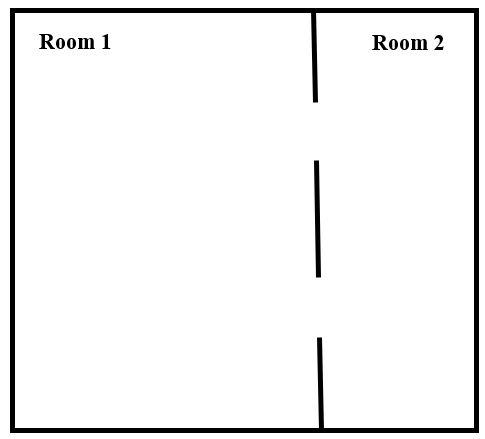
\includegraphics[width=.5\linewidth]{images/img1.JPG} 
    \caption{No goal} 
    \vspace{4ex}
  \end{subfigure}%%
  \begin{subfigure}[b]{0.5\linewidth}
    \centering
    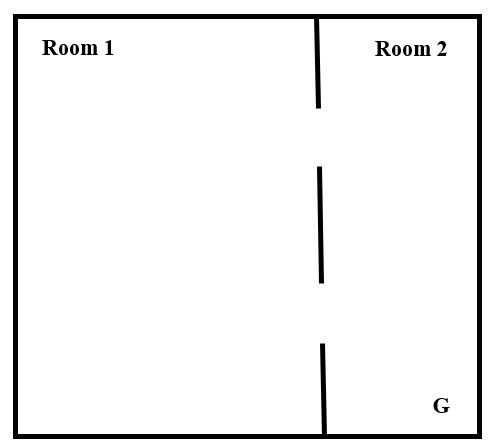
\includegraphics[width=.5\linewidth]{images/img2.JPG} 
    \caption{Goal in Room 2} 
    \vspace{4ex}
  \end{subfigure} 
  \begin{subfigure}[b]{0.5\linewidth}
    \centering
    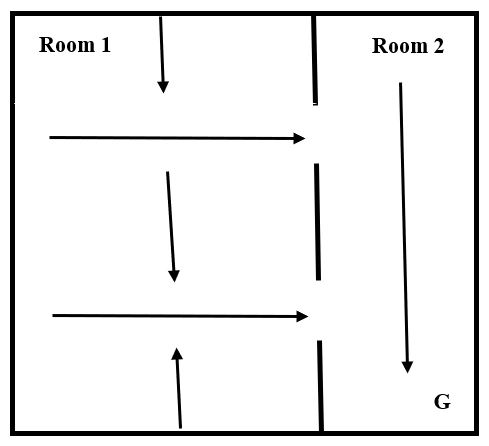
\includegraphics[width=.5\linewidth]{images/img3.JPG} 
    \caption{Hierarchically Optimal Solution} 
    \vspace{4ex}
  \end{subfigure}%% 
  \begin{subfigure}[b]{0.5\linewidth}
    \centering
    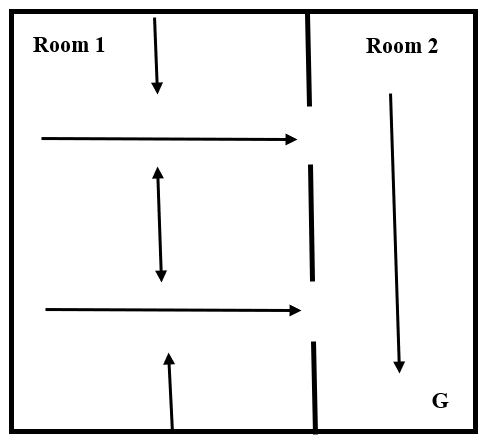
\includegraphics[width=.5\linewidth]{images/img4.JPG} 
    \caption{Recursively Optimal Solution} 
    \vspace{4ex}
  \end{subfigure} 
    \caption{Example to illustrate optimality}

\end{figure}




\subsection{Hierarchical Optimality}

A policy is hierarchically optimal if it is the most optimal amongst all the policies that respect the hierarchy. Such a solution need not be optimal on each of its subproblems. As evident from Fig 1(c), the agent in this case tries to make its way out of Room 1 maximizing his prospects of reaching the goal in the best possible way. In other words, in hierarchical optimality the presence of hierarchy is respected and is strictly adhered to. On the other hand, a recursive optimality keeps in mind the hierarchy but alters it to prioritize the subtasks first. As the overall hierarchy is put forth first, a solution with hierarchical optimality is always lesser than that of recursive optimality. Despite the con, recursive optimality gives the payoff of modularity. 

Consider a laser beam midway in Room 2, which destroys the agent completely. Due to its immense negative impact, an extremely negative reward is kept aside for crossing the beam. Despite this high negative reward, the recursively optimal solution remains the same for Room 1. However, a hierarchically optimal solution makes sure that the agent is always directed towards the lower passage in Room 1. For this extended example, the hierarchical solution has an upper hand over the recursive one. 


\subsection{Flat Optimality}

Unlike the other two optimalitys, a flat solution does not respect hierarchy. It simply yields us the solution which is globally the most optimal. It might not even compute the solutions to the individual subproblems. 
